%!tex root = ../main.tex

%\section{Automatically proving lower bounds for LCL problems} \label{sec:implementation}
\section{Implementation} \label{sec:implementation}
In this section we will cover all the important topics that are used in the actual implementation of the Algorithm~\ref{alg:counterexample_finder} from Section~\ref{sec:algorithm}.
This includes the previously declared functions $\textsc{SolutionExists}(\Pi, g)$ and $\textsc{GenerateGraphs}(n, d_a, d_p)$, which were given as black boxes.
In Section~\ref{}, we discuss 
In Section~\ref{}, we discuss how we generate multigraphs.
In Section~\ref{}

The implementation itself is a computer program~\cite{NonconstantLclClassifier2022}, that attempts to automatically find a proof of unsolvability for an LCL problem in PN model.
Although the implementation is programmed in Rust programming language~\cite{RustLang}, we keep the explanations independent of any programming language.

The function $\textsc{SolutionExists}(\Pi, g)$ checks if an LCL problem $\Pi$ is unsolvable in some $(d_a, d_p)$-biregular multigraph $g$.
To perform the checking, it is enough to show that there exists no valid labeling of $\Pi$ in $g$.
In the implementation this is done with following steps:
\begin{enumerate}
    \item encode the problem $\Pi$ and multigraph $g$ into a SAT problem $S$,
    \item solve the problem $S$ using some efficient SAT solver.
\end{enumerate}
When we feed the SAT problem $S$ into a SAT solver, we get either SAT (satisfiable) or UNSAT (unsatisfiable) as a result.
In case the result is UNSAT, the SAT solver found no possible labeling for the problem.
Thus we have found a counterexample and we are done.
Otherwise we can continue searching using some other multigraph.
The routine is illustrated on Figure \ref{fig:implementation:1}.

\begin{figure}[H]
\centering
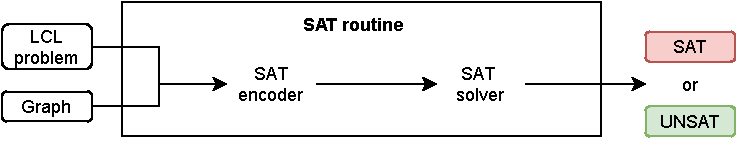
\includegraphics[]{diagrams/implementation_idea_diagram2.pdf}
\caption{The SAT routine. When given a multigraph and an LCL problem, it checks if a valid labeling exists.}
\label{fig:implementation:1}
\end{figure}

We repeat the routine for each multigraph, as shown in the Algorithm \ref{alg:counterexample_finder}, and terminate early if the result is UNSAT.
\todo{WIP}

\begin{figure}[H]
\centering
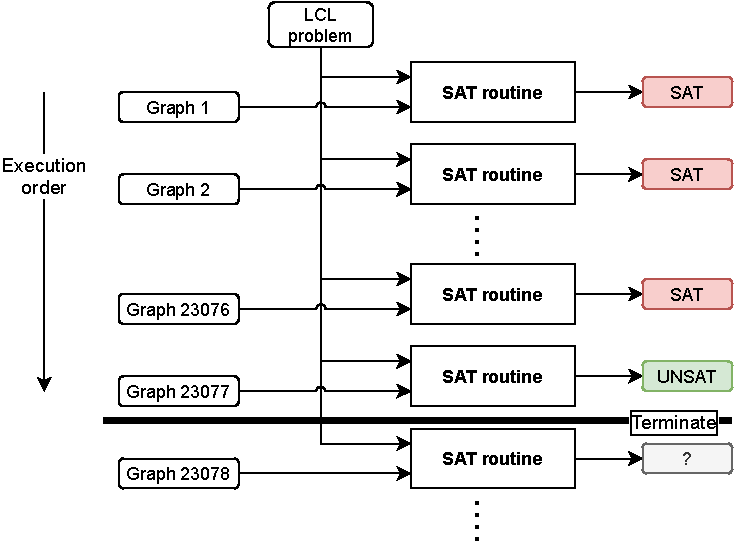
\includegraphics[]{diagrams/implementation_idea_diagram3.pdf}
\caption{An example of an execution of multiple SAT routines. Execution terminates at graph $77$ when first UNSAT is encountered.}
\label{fig:implementation:2}
\end{figure}

%TODO biregular multigraphs?
%TODO LCL problems on biregular trees etc?

%When we assume that an LCL problem $\Pi$ is solvable in PN, we mean that there exists a deterministic distributed algorithm $A$ in PN model, that finds a solution for all multigraphs i.e. algorithm $A$ works in every multigraph.
%Every simple graph is also a multigraph, thus multigraphs are more relaxed in terms of definition.
%Allowing parallel edges potentially gives us counterexamples with smaller graph sizes when we use the increasing strategy i.e. our algorithm might terminate succesfully much earlier with the desired result and graphs do not necessarily become as complex as they would be with only simple graphs.
%%TODO where to discuss about solutions that have been found only with multigraphs? Have we found any solutions with only simple graphs?
%Smaller graphs mean less complexity and less performance required but as there are also more graphs to iterate, it is not so simple to justify allowing parallel edges only with this argument.
%The main argument is that allowing parallel edges gives us more opportunities to find counterexamples.
%It might be that in some problems we cannot even find counterexamples without parallel.

%This is indeed what we have used in this work.
%Probably, we have to iterate a lot of graphs.
%For this purpose we want to be able to generate the graphs.



\subsection{Generating multigraphs}
We want to generate $(\Delta, \delta)$-biregular multigraphs, but how can we do it?
A naive approach to this would be generating all possible graphs, and then filtering out graphs that are not in the graph family.
This is a very bad idea, and we show why.

Let us first consider only simple graphs.
We need to figure out the formula for the number of simple graphs with $n$ vertices.
A complete graph of $n$ vertices has an edge between any two vertices.
The count of edges in a complete graph is \(\binom{n}{2} = \frac{n!}{2!(n-2)!} = \frac{n(n-1)}{2}.\)
Therefore, there are \(2^{\frac{n(n-1)}{2}}\) different simple graphs of size $n$, as there are two options for each edge, either they are in the graph or not.
The number of simple graphs grows exponentially fast, as shown in Table~\ref{tbl:graph_count_growth}.
This is clearly too much for modern computers with small numbers of $n$, therefore we need to think of better options.
%0, 1, 3, 6, 10, 15, 21, 28, 36, 45, 55,
%1, 2, 8, 64, 1024, 32768, 2097152, 268435456, 68719476736, 35184372088832, 36028797018963968
\begin{table}[H]
  \centering
  \begin{tabular}{r|rr}
    \toprule
    $n$&Edges&Graphs\\
    \midrule
    1 & 0 &1\\
    2 & 1 &2\\
    3 & 3 &8\\
    4 & 6 &64\\
    5 & 10 &1024\\
    6 & 15 &32768\\
    7 & 21 &2097152\\
    8 & 28 &268435456\\
    9 & 36 &68719476736\\
    10 & 45 &35184372088832\\
    11 & 55 &36028797018963968\\
    \vdots & \vdots &\vdots\\
    \bottomrule
  \end{tabular}
  \caption{
    A list of number of edges in complete graphs, and the number of simple graphs.
  }
  \label{tbl:graph_count_growth}
\end{table}

In this experiment we did not even consider multiple edges.
With multiple edges without any limits, the number of multigraphs is infinite.
However, this is not true when we consider only $(\Delta, \delta)$-biregular multigraphs of size $n$.
Clearly the number of multiple edges is bounded by $\max(\Delta, \delta)$.

The numbers of incident edges for nodes of parts $A$ and $B$ are $\Delta$ and $\delta$, respectively.
We know from Equation~\ref{eq:biregular:sum_of_degrees} that the sums of degrees of each node in each part must be equal.
How do we know the number of nodes in each part i.e. what are the possible pairs of positive integers that sum up to $n$?
There are only $n-1$ possibilities:
$$(1, n-1), (2, n-2), ..., (n-2, 2), (n-1, 1).$$
Out of those pairs, only pairs $(n_A, n_B)$ such that
\begin{equation} \label{eq:pairs:1}
  \Delta n_A = \delta n_B,
\end{equation}
\begin{equation} \label{eq:pairs:2}
n_A + n_B = n
\end{equation}
will work.
If we assume that $\Delta \geq \delta$, then we can see from Equation~\ref{eq:pairs:1} that $n_A\leq n_B$, therefore we only need to consider pairs

$$(1, n-1), (2, n-2), ..., (\left\lfloor\frac{n}{2}\right\rfloor, n - \left\lfloor\frac{n}{2}\right\rfloor).$$

For example with $(3,2)$-biregular multigraphs, we can only have the pair $(4, 6)$, as shown in Table~\ref{tbl:possible_pairs}.
However, most of the time there are no valid pairs for chosen $n$, as we can see for $n=9$ in Table \ref{tbl:possible_pairs:no_pairs}.

\begin{table}[H]
  \parbox{.45\linewidth}{
    \centering
    \begin{tabular}{rrrr}
    \toprule
    $n_A$&$n_B$&$\Delta n_A$&$\delta n_B$\\
    \midrule
    1 & 9 & 3  & 18\\
    2 & 8 & 6  & 16\\
    3 & 7 & 9  & 14\\
    \textbf{4} & \textbf{6} & \textbf{12} & \textbf{12}\\
    5 & 5 & 15 & 10\\
    \bottomrule
  \end{tabular}
  \caption{
    Possible pairs of node counts for part A and B in a $(3,2)$-biregular multigraph when $n=10$.
    The only valid pair with $\Delta n_A = \delta n_B$ is (4, 6), and it is bolded.
  }
  \label{tbl:possible_pairs}
  }
  \hfill
  \parbox{.45\linewidth}{
  \centering
  \begin{tabular}{rrrr}
    \toprule
    $n_A$&$n_B$&$\Delta n_A$&$\delta n_B$\\
    \midrule
    1 & 8 & 3  & 16\\
    2 & 7 & 6  & 14\\
    3 & 6 & 9  & 12\\
    4 & 5 & 12 & 10\\
    \bottomrule
  \end{tabular}
  \caption{
    Possible pairs of node counts for part A and B in a $(3,2)$-biregular multigraph when $n=9$.
    There are no valid pairs.
  }
  \label{tbl:possible_pairs:no_pairs}
  }
\end{table}

It turns out that there is always at most one pair that fills the conditions shown in Equations~\ref{eq:pairs:1} and \ref{eq:pairs:2}.
We can find a formula for all possible values of n
\begin{align}
  n_A &= x \\
  n_B &= n-x\\
  \Delta x &= \delta (n-x) \\
  \Rightarrow n&=\frac{x(\Delta+\delta)}{\delta}\\
\end{align}

When we fix $\Delta$ and $\delta$, the possible numbers for $n$ are all integers $\frac{x(\Delta + \delta)}{\delta}$, where $x$ is any positive integer.
Not necessarily all values of $x$ result on an integer, but this is more than enough.
We can iterate through all $x$ up to some upper bound, and consider only values of $n$ that are integers, as we do in Table \ref{tbl:values_of_x}.
We then compute all valid pairs of $(n_A, n_B)$ in Table \ref{tbl:valid_pairs}.
%Thus, we get equations $n_A=\Delta x$ and $n_B=\delta x$.
%For example, we list all valid pairs for $(3, 2)$-biregular multigraphs in Table~\ref{tbl:valid_pairs}.

\begin{table}[H]
  \parbox{.45\linewidth}{
  \centering
  \begin{tabular}{rr}
    \toprule
    $x$&$n=\frac{x(\Delta + \delta)}{\delta}$\\
    \midrule
    1 & 2.5 \\
    \textbf{2} & \textbf{5}   \\
    3 & 7.5 \\
    \textbf{4} & \textbf{10}  \\
    \vdots & \vdots \\
    \bottomrule
  \end{tabular}
  \caption{
    All values of $x$ and $n$ for $(3,2)$-biregular multigraph.
    All rows where $n$ is an integer, are bolded.
  }
  \label{tbl:values_of_x}
  }
  \hfill
  \parbox{.45\linewidth}{
  \centering
  \begin{tabular}{rrr}
    \toprule
    $n$&$n_A=x$&$n_B=n-x$\\
    \midrule
    5 & 2 & 3   \\
    10 & 4 & 6  \\
    15 & 6 & 9  \\
    20 & 8 & 12 \\
    \vdots & \vdots & \vdots\\
    \bottomrule
  \end{tabular}
  \caption{
    All valid $n$ and pairs of $(n_A, n_B)$ for $(3,2)$-biregular multigraph.
  }
  \label{tbl:valid_pairs}
  }
\end{table}

Now we know a lot more about the graphs we are going to generate.
Given that we know $\Delta$ and $\delta$, we can easily generate all possible graph sizes for $(\Delta, \delta)$-biregular multigraphs.

Before we tell more about the function $\textsc{GenerateGraphs}(n, d_a, d_p)$, we want to discuss graph isomorphism.
We quote the definition of graph isomorphism from~\cite{DBLP:journals/jsc/McKayP14}:
\begin{displayquote}
An isomorphism between two graphs is a bijection between their vertex sets that preserves adjacency.
\end{displayquote}
In other words, they are similar because of symmetry.
To decrease the number of graphs drastically, we are interested only in nonisomorphic graphs i.e. there is no similarity between any two graphs.
There is a well known software package called \emph{nauty and Traces}~\cite{DBLP:journals/jsc/McKayP14}, that has tools for generating all nonisomorphic graphs of different graph families.
The collection of tools is called \emph{gtools}.
In Table \ref{tbl:graph_count_nonisomorphic}, we show the count of simple graphs, as in Table~\ref{tbl:graph_count_growth}.
Alongside the values, we show the count of nonisomorphic simple graphs.
As we can see, there are significantly fewer nonisomorphic simple graphs than there are simple graphs.
Thus, we want to generate only nonisomorphic graphs.
For our implementation of $\textsc{GenerateGraphs}(n, d_a, d_p)$, we use the tools \emph{genbg} and \emph{multig} from gtools.

\begin{table}[H]
  \centering
  \begin{tabular}{r|rrrr}
    \toprule
    $n$&Simple graphs & Nonisomorphic simple graphs & Time (s)\\
    \midrule
    1  &1                 & 1 & 0.00\\
    2  &2                 & 2 & 0.00\\
    3  &8                 & 4 & 0.00\\
    4  &64                & 11 & 0.00\\
    5  &1024              & 34 & 0.00\\
    6  &32768             & 156 & 0.00\\
    7  &2097152           & 1044 & 0.00\\
    8  &268435456         & 12346 & 0.00\\
    9  &68719476736       & 274668   & 0.09\\
    10 &35184372088832    & 12005168 & 3.57\\
    11 &36028797018963968 &1018997864&295.13\\
    \vdots & \vdots &\vdots\\
    \bottomrule
  \end{tabular}
  \caption{%
    The numbers of simple graphs, and nonisomorphic simple graphs.
    There is also generation time for each nonisomorphic set of simple graphs.
    Nonisomorphic graphs were generated with the tool called \emph{geng}.
    The tool was executed on a single thread of AMD Ryzen 9 3900X 12-Core Processor.
    For example, the command for generating all 10-sized connected simple graphs is \codee{geng 10 > simple10.txt}.
  }
  \label{tbl:graph_count_nonisomorphic}
\end{table}

The first tool, genbg, is used to generate small bipartite graphs that are nonisomorphic.
The tool requires number of vertices for parts A and B separately, and we already know how to generate them.
We additionally specify two ranges of degrees so that we get bipartite graphs, where the degrees of nodes range from $1$ to $\Delta$ and from $1$ to $\delta$ in parts A and B, respectively.
We also use a flag ``-c'' to generate only connected graphs.
The output from the graph is then fed into the second tool.

The second tool, multig, is used to generate small multigraphs with a given underlying graph.
It replaces edges of a simple graph with multiple edges in all possible ways.
All graphs outputted from multig are also nonisomorphic.
The tool takes an exact range of edges we want for the graphs, and we already know that the number is exactly $\Delta n_A = \delta n_B$.
We also give the tool a maximum edge multiplicity of $\Delta$ and upper bound of $\Delta$ on maximum degree, as we assume that $\Delta \geq \delta$.
By feeding the bipartite graphs from genbg to multig, we will receive $(\Delta, \delta)$-biregular multigraphs.
The output format from multig is a simple text format that is quite trivial to parse, so we do not discuss more about it.

\todo{Discuss something about Table~\ref{tbl:graph_count_nonisomorphicasdasd}}

\begin{table}[H]
  \centering
  \begin{adjustbox}{width={\textwidth},keepaspectratio}%
  \begin{tabular}{r|rr|rr|rr}
    \toprule
    $n$& $n_A$ & $n_B$ & Simple bipartite graphs & Time (s) & (3,2)-biregular multigraphs  & Time (s)\\
    \midrule
    %&&&&& \multicolumn{2}{c}{Trees} \\
    %Classifier & Complete & Labels & Paths & Cycles &Rooted & Unrooted \\\midrule
    5   & 2 & 3   & 4  & 0.00    & 4     & 0.00\\
    10  & 4 & 6   & 24  & 0.00   & 42    & 0.00\\
    15  & 6 & 9   & 272  & 0.01  & 658   & 0.00\\
    20  & 8 & 12  & 4146 & 0.23  & 13902 & 0.04\\
    25  & 10 & 15 & 79052 & 7.60 & 357219& 1.37\\
    \vdots & \vdots &\vdots&\vdots&\vdots&\vdots&\vdots\\
    \bottomrule
  \end{tabular}
  \end{adjustbox}
  \caption{%
    The counts of simple bipartite graphs and (3,2)-biregular multigraphs, when $(\Delta, \delta) = (3, 2)$.
    Both graph families are connected and nonisomorphic.
    We used the tools genbg and multig, as discussed above, and we feed the output from genbg to multig.
    We also show the time it takes to generate each set of graphs.
    The tools were executed on a single thread of AMD Ryzen 9 3900X 12-Core Processor.
  }
  \label{tbl:graph_count_nonisomorphicasdasd}
\end{table}


\subsection{Generating LCL problems}

When we generate LCL problems, we generate whole class of LCL problems.
A class of LCL problems is a set of LCL problems where the problems share common attributes.
The attributes are the values of a triple $(\Delta, \delta, l)$, where $\Delta$ and $\delta$ are the sizes of a label configuration in $A$ and $P$, respectively, and $l$ is the size of $\Sigma$ i.e. the number of labels.

The set of all possible label configurations is a $k$-combination with repetitions, where $k$ is the size of a label configuration.
Let us call the function of $k$-combination with repetitions as $\operatorname{comb}(k, \Sigma)$.
For example, if $\Delta$ is 2, $\Sigma=\{A, B\}$ and $l$ is 2, then the set of all possible label configurations is
$$ \operatorname{comb}(\Delta, \Sigma) = \{ \{A, A\}, \{A, B\}, \{B, B\} \}. $$

The set of all possible sets of label configurations is a power set of the set of all possible label configurations, excluding an empty set.
Let us call this power set without an empty sets as a function $\operatorname{pow}(d, S)$, where $d$ is the size of a label configuration, and $S$ is the set of all possible label configurations.
For example, the power set of above example excluding an empty set is
\begin{align*}
  \operatorname{pow}(\Delta, \operatorname{comb}(\Delta, \Sigma)) =  \{&\{\{A, A\}\}, \\
    &\{\{A, B\}\}, \\
    &\{\{B, B\}\}, \\
    &\{\{A, A\}, \{A, B\}\}, \\
    &\{\{A, A\}, \{B, B\}\}, \\
    &\{\{A, B\}, \{B, B\}\}, \\
    &\{\{A, A\}, \{A, B\}, \{B, B\}\} \}.\\
\end{align*}

The set of all LCL problems of class $(\Delta, \delta, l)$ is a Cartesian product
$$ \operatorname{comb}(\Delta, \Sigma) \times \operatorname{comb}(\delta, \Sigma),$$
where $\Sigma$ is any set of labels of length $l$.
In our implementation, we use the upper-case alphabet as $\Sigma$.
The elements are pairs $(A, P)$, where $A$ is the set of all allowed label configurations for active nodes, and $P$ is the set of all allowed label configurations for passive nodes.

Now that we know how to generate a class of LCL problems, we want to show the number of elements in some classes.
See Table \ref{}.

\begin{table}[H]
  \centering
  \begin{tabular}{r|rrrr}
    \toprule
    $n$&Simple graphs & Nonisomorphic simple graphs & Time (s)\\
    \midrule
    1  &1                 & 1 & 0.00\\
    2  &2                 & 2 & 0.00\\
    3  &8                 & 4 & 0.00\\
    4  &64                & 11 & 0.00\\
    5  &1024              & 34 & 0.00\\
    6  &32768             & 156 & 0.00\\
    7  &2097152           & 1044 & 0.00\\
    8  &268435456         & 12346 & 0.00\\
    9  &68719476736       & 274668   & 0.09\\
    10 &35184372088832    & 12005168 & 3.57\\
    11 &36028797018963968 &1018997864&295.13\\
    \vdots & \vdots &\vdots\\
    \bottomrule
  \end{tabular}
  \caption{%
    The numbers of simple graphs, and nonisomorphic simple graphs.
    There is also generation time for each nonisomorphic set of simple graphs.
    Nonisomorphic graphs were generated with the tool called \emph{geng}.
    The tool was executed on a single thread of AMD Ryzen 9 3900X 12-Core Processor.
    For example, the command for generating all 10-sized connected simple graphs is \codee{geng 10 > simple10.txt}.
  }
  \label{tbl:graph_count_nonisomorphic}
\end{table}



Let us first talk about the format we use to represent LCL problems.
In Section~\ref{}, we showed the maximal independent set problem in infinite (3,2)-biregular graphs.
We represent the problem in the format as follows:
\todo{Tell how we generate all LCL problems}

\todo{tell how we normalize problems}
\todo{tell about purging}



\subsection{Boolean satisfiability problem}
\todo{Explain
\begin{itemize}
  \item SAT problems, %TODO
  \item DIMACS CNF, %TODO
  \item SAT solvers, %TODO
\end{itemize}
}

\subsection{SAT solvers} % talk about sats generally before talkign specifically how we encode the problems

\subsection{SAT encoding and solving}

\todo{Use the section 4.1 ``SAT encoding'' from \cite{DBLP:conf/sat/JarvisaloKKK12} as an inspiration for this section. Maybe we will find a nice way to present things?}

%\subsection{Software optimizations
\subsection{Caching}
%TODO pre-computing multigraphs and lcl problems and saving them?

\subsection{parallelization}
%TODO Talk about parallelization here or separately in above sections

